\documentclass{beamer}
\mode<presentation> {
% The Beamer class comes with a number of default slide themes
% which change the colors and layouts of slides. Below this is a list
% of all the themes, uncomment each in turn to see what they look like.

%\usetheme{default}
%\usetheme{AnnArbor}
%\usetheme{Antibes}
%\usetheme{Bergen}
%\usetheme{Berkeley}
%\usetheme{Berlin}
%\usetheme{Boadilla}
%\usetheme{CambridgeUS}
%\usetheme{Copenhagen}
%\usetheme{Darmstadt}
%\usetheme{Dresden}
%\usetheme{Frankfurt}
%\usetheme{Goettingen}
%\usetheme{Hannover}
%\usetheme{Ilmenau}
%\usetheme{JuanLesPins}
%\usetheme{Luebeck}
\usetheme{Madrid}
%\usetheme{Malmoe}
%\usetheme{Marburg}
%\usetheme{Montpellier}
%\usetheme{PaloAlto}
%\usetheme{Pittsburgh}
%\usetheme{Rochester}
%\usetheme{Singapore}
%\usetheme{Szeged}
%\usetheme{Warsaw}
\usepackage{fancyhdr}
\usepackage{animate}
\usepackage{caption}
\usepackage{subcaption}
\usepackage{hyperref}

% As well as themes, the Beamer class has a number of color themes
% for any slide theme. Uncomment each of these in turn to see how it
% changes the colors of your current slide theme.

%\usecolortheme{albatross}
%\usecolortheme{beaver}
%\usecolortheme{beetle}
%\usecolortheme{crane}
%\usecolortheme{dolphin}
%\usecolortheme{dove}
%\usecolortheme{fly}
%\usecolortheme{lily}
%\usecolortheme{orchid}
%\usecolortheme{rose}
%\usecolortheme{seagull}
%\usecolortheme{seahorse}
%\usecolortheme{whale}
%\usecolortheme{wolverine}

%\setbeamertemplate{footline} % To remove the footer line in all slides uncomment this line
\setbeamertemplate{footline}[page number] % To replace the footer line in all slides with a simple slide count uncomment this line

\setbeamertemplate{navigation symbols}{} % To remove the navigation symbols from the bottom of all slides uncomment this line
}

\usepackage{graphicx} % Allows including images
\usepackage{booktabs} % Allows the use of \toprule, \midrule and \bottomrule in tables
\usepackage{multirow} % Allows use of multirow
%\usepackage {tikz}
\usepackage{tkz-graph}
\GraphInit[vstyle = Shade]
\tikzset{
  LabelStyle/.style = { rectangle, rounded corners, draw,
                        minimum width = 2em, fill = yellow!50,
                        text = red, font = \bfseries },
  VertexStyle/.append style = { inner sep=5pt,
                                font = \normalsize\bfseries},
  EdgeStyle/.append style = {->, bend left} }
\usetikzlibrary {positioning}
%\usepackage {xcolor}
\definecolor {processblue}{cmyk}{0.96,0,0,0}
%----------------------------------------------------------------------------------------
%	TITLE PAGE
%----------------------------------------------------------------------------------------

\title[Short title]{Particle Filter based SLAM} % The short title appears at the bottom of every slide, the full title is only on the title page

\author{Aswin P Ajayan} % Your name
\institute[Indian Institute of Technology, Bombay] % Your institution as it will appear on the bottom of every slide, may be shorthand to save space
{
Indian Institute of Technology, Bombay\\ % Your institution for the title page
\medskip
}
\date{Jun 30, 2020} % Date, can be changed to a custom date

\begin{document}

\begin{frame}
\titlepage % Print the title page as the first slide
\end{frame}

\begin{frame}
\frametitle{Overview} % Table of contents slide, comment this block out to remove it
\tableofcontents % Throughout your presentation, if you choose to use \section{} and \subsection{} commands, these will automatically be printed on this slide as an overview of your presentation
\end{frame}

%----------------------------------------------------------------------------------------
%	PRESENTATION SLIDES
%----------------------------------------------------------------------------------------

%------------------------------------------------

\section{What is SLAM}
\begin{frame}{What is SLAM}
    \begin{itemize}
    \item Computing robot's poses and map environment simultaneously \\
    \item Localisation : estimating robots location\\ 
    \item Mapping      : building a MAP\\
    \item Given
    \begin{itemize}
        \item $u_{1:T} = \{u_1,u_2,u_3....u_T\}$, the control inputs
        \item $z_{1:T} = \{z_1,z_2,z_3,...,z_T\}$, observations

    \end{itemize}
\item Wanted
    \begin{itemize}
    \item $m$, map of the environment
    \item $x_{0:T} = \{x_0,x_1,x_2,...,x_T\}$ , robot location
    \item $p(x_{0:T},m | u_{0:T},z_{1:T})$, the SLAM posterior
        \end{itemize}
\end{itemize}


\end{frame}


\section{Objective}
\begin{frame}{Objective}
    \begin{itemize}
        \item To review the literature available on SLAM. To get acquainted with various techniques available for SLAM and examine some of them in depth. Simulation in reallife constraints using ROS.\\
            Types of SLAM techniques explored includes
        \item \textbf{Kalman Filter based approaches}
            \begin{itemize}
                \item Extended Kalman Filter
                \item Unscented Kalman Filter
                \item Extended Information Filter
            \end{itemize}
            \item \textbf{Particle Filter based approaches}
                \begin{itemize}
                    \item Fast SLAM -Rao Blackwellised Particle Filter
                        \begin{itemize}
                            \item Augmented MCL
                        \end{itemize}
                \end{itemize}
       \end{itemize}
\vfill
\end{frame}


\section{Types of SLAM}
\begin{frame}{Types of SLAM}
    \begin{itemize}
        \item Full SLAM vs online SLAM
        \begin{itemize}
            \item Full SLAM $p(x_{0:T},m|u_{1:t},z_{1:t})$
            \item Full SLAM $p(x_{t},m|u_{1:t},z_{1:t})$
        \end{itemize}
        \item Feature Based SLAM vs Grid Based
\begin{figure}
     \centering
        \begin{subfigure}[b]{0.4\textwidth}
        % \centering
        \hspace*{-10mm}
        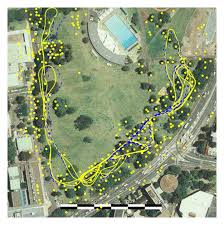
\includegraphics[height = 40mm,width = 60mm]{feature_maps.jpeg}
        \end{subfigure}
    ~
        \begin{subfigure}[b]{0.4\textwidth}
        \centering
        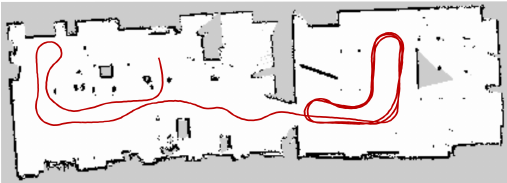
\includegraphics[height = 40mm,width = 60mm]{gridMap.png}
        \end{subfigure}
    \end{figure}   

        \item Active SLAM vs Passive SLAM
    \end{itemize}
\end{frame}


\section{Markov assumption and Recursive Bayesian estimate}
\begin{frame}{Recursive Bayesian Estimation}
    \begin{itemize} 
        \item \textbf{Markov assumption} : next state depends only on the present state
            $$p(x_{t}|x_{0:t},u_{1:t}) = p(x_t | x_{t-1},u{t})$$
        \item \textbf{Recursive Bayesian Estimation}
\begin{align*}  
    bel(x_t) & = p(x_t | z_{1:t},u_{1:t})\\
    & = \eta p(z_t|x_t) \int_{x_{t-1}} p(x_t |x_{t-1},u_t) * bel(x_{t-1})dx_{t-1}
 \end{align*}
 we can split this into predict and update steps where\\
 \textbf{Predict Step} 
 $$\overline{bel(x_t)} =  \int_{x_{t-1}} p(x_t |x_{t-1},u_t) * bel(x_{t-1})dx_{t-1}$$
 \textbf{Update Step} 
 $$bel(x_t) =  \eta * p(z_t | x_t) * \overline{bel(x_t)}$$


 \textbf{Bayes filter} recursive estimation is realised using kalman filter, Information Filter, particle filter etc.
    \end{itemize}
\end{frame}

\section{Frameworks for recursive filter estimation}
\begin{frame}{Kalman Filter Family}
    Beliefs are represented in parametric form 
    with mean vector $\mu_t$ and covariance matrix $\Sigma _t$ . Closed form expressions are available for belief propagation under certain cases

    \begin{itemize}        
        \item \textbf{Kalman Filter :} Assumes linear models(state transistion and measurement) and gaussian posterior
        \item \textbf{Extended Kalman Filter :} Linearises the model and then applies normal KF
        \item \textbf{Unscented Kalman Filter :} Samples a gaussian posterior from the resulting non linear transformation
        \item \textbf{Information Filters :} Uses canonical representaion of Belief i.e. $\mu_{t}^{-1}$ and $\Sigma_{t}^{-1}$
    \end{itemize}
\end{frame}


\section{Particle Filters}
\begin{frame}{Particle Filter}
    \begin{itemize}
        \item Use particles to represent instead of parametric models.
        \item Can effectively model mutli modal distributions . 
        \item Can Take care of the non linearities in the model  
        \item Computationally intensive
        \item Based on importance sampling principal 
    \end{itemize}
\end{frame}


\begin{frame}{Particle filter}
    \textbf{Importance Sampling} - Use to generate samples from an arbitrary distribution\\
    \begin{figure}
        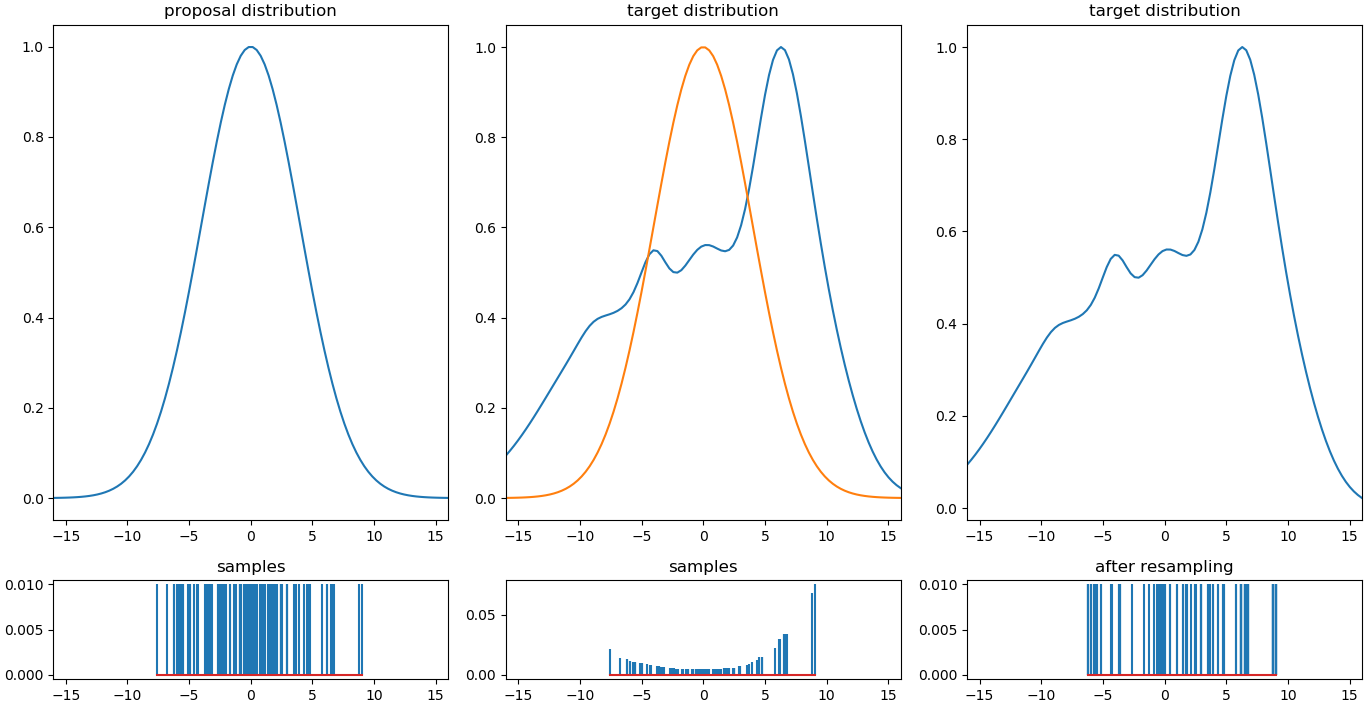
\includegraphics[height = 30mm, width = 80mm]{./importance_sampling.png}
    \end{figure}
    \textit{steps}
    \begin{itemize}
        \item Draw samples from a proposal distribution
        \item calculate the importance weight as $ w_t^{[j]} = \frac{target(x_t^{[j]})}{proposal(x_t^{[j]})}$
        \item Resample based on weights
    \end{itemize}
\tiny{$^{4}$} https://github.com/aswinpajayan/seminar-related/scripts/importance sampling.py
\end{frame}


\begin{frame}{Particle filter}
            \begin{itemize}
                \item sampling from proposal distribution : 
                    $$x_t^{[j]} \sim \pi(x_t|x_{t-1},u_{t-1})$$
                \item Importance weighting :
                    $$ w_t^{[j]} = \frac{target(x_t^{[j]})}{proposal(x_t^{[j]})} = p(z_t|x_t) $$
                \item Resampling : Draw sample $i$ with probability $w_t^{[j]}$
            \end{itemize}

\tiny{$^{1}$} Source: Probabilistic Robotics, Sebastian Thrun
\end{frame}

\section{RBPF}
\begin{frame}{Rao-Blackwellisation for SLAM - Fast SLAM 1.0}
    \begin{itemize}
        \item Particle filters are ideal for low dimensional states i.e. $|| x_t ||$ is small.
        \item for SLAM problem, Number of landmarks may be very large. So Particle filter cant be used directly
        \item Estimate the pose using particle filter and then compute map. 
\begin{align*}
    p(a,b) & = p(b|a).p(a)\\
    \sim p(x_{0:t},m_{1:M}|z_{1:t},u_{1:t}) & =  p(x_{0:t}|z_{1:t},u_{1:t}).p(m_{1:M}|z_{1:t},u_{1:t})\\
    & =  p(x_{0:t}|z_{1:t},u_{1:t}) \Pi p(m_{i}|z_{1:t},u_{1:t})\\
\end{align*}
Now each particle respresents a path hypothesis and it has an assosicated map with it. Splitting $p(m_{1:M})$ into $\Pi p(m_i)$ reduces the computational complexity further, each of this is calculated by a 2x2 EKF. 
\newline 
    \end{itemize}
\end{frame}


\begin{frame}{RBPF particle structure}
    Each particle maintains M 2x2 EKF along with the 3 pose variables 
\begin{figure}
    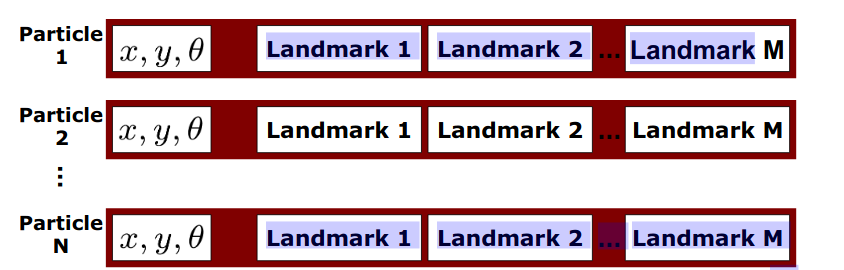
\includegraphics[width = \linewidth]{./RBPF_particles.png}
    \caption{Particle structure in RBPF-slam}
\end{figure}

\end{frame}

\section{Implementing Particle filter localisation}
\begin{frame}{Implementing Particle filter localisation}
    \begin{itemize}
        \item \textbf{Simulation Platform: } - ROS melodic Ubuntu 18.04 
        \item \textbf{Robot: } - Custom robot using URDF
        \begin{itemize}
            \item motion model libgazebo\_ros\_diff\_drive.so 
            \item sensor model head\_hokuyo\_sensor
        \end{itemize}
        \item \textbf{Visualisation: } - matplot lib interactive plots , python 2.7
    \end{itemize}
\end{frame}

\subsection{Creating a custom robot}
\begin{frame}{Creating a custom robot}
    \begin{figure}
        \centering
        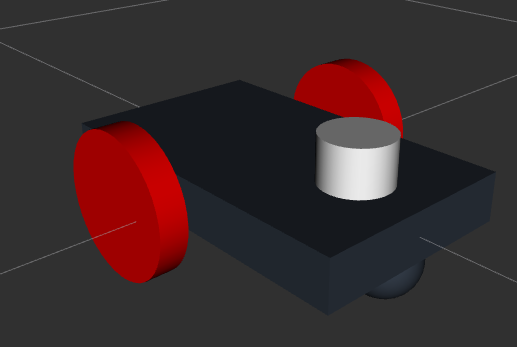
\includegraphics[height=30mm]{./custom_robot.png}
    \end{figure}
    \begin{itemize}
    \item \textit{Universal Robot Description Format} provides an easy way to create a custom meshes for a robot. The motion model and sensor model are realised using the gazebo plugins. The robot was created using xacro files: which stands for XML Macros. 
    \item sensor: Laser range finder with standard deviation 0.01 and gaussian model was used
    \end{itemize}
    \vfill
    \tiny{$^{3}$} https://www.theconstructsim.com/ros-projects-exploring-ros-using-2-wheeled-robot-part-1/
\end{frame}

\subsection{Creating a motion model}
\begin{frame}{Creating a motion model}
    \begin{itemize}
        \item Particle filter uses a motion model as the proposal distribution and sensor model for inferring importance weights 
        \item  A simple motion model was used :\\
            $$x_t = x_{t-1} + v.cos(\theta_{t-1})$$
            $$y_t = y_{t-1} + v.sin(\theta_{t-1})$$
            $$\theta _t = \theta _{t-1} + w \delta _{t}$$
        v, w are linear velocity, angular velocity. 
    \end{itemize}
\end{frame}

\subsection{creating a sensor model}
\begin{frame}{Creating a sensor model}
    \begin{itemize}

        \item Maximum likelihood field was chosen to be used as the sensor model 
        \item The field was generated using a convolution with a kernel and point landmark map.
\begin{figure}


     \centering
        \begin{subfigure}[b]{0.4\textwidth}
        % \centering
        \hspace*{-10mm}
        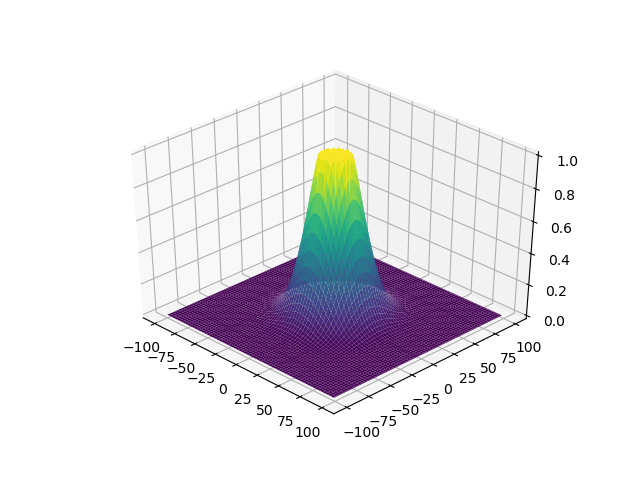
\includegraphics[height = 40mm,width = 60mm]{kernel.png}
        \end{subfigure}
    ~
        \begin{subfigure}[b]{0.4\textwidth}
        \centering
        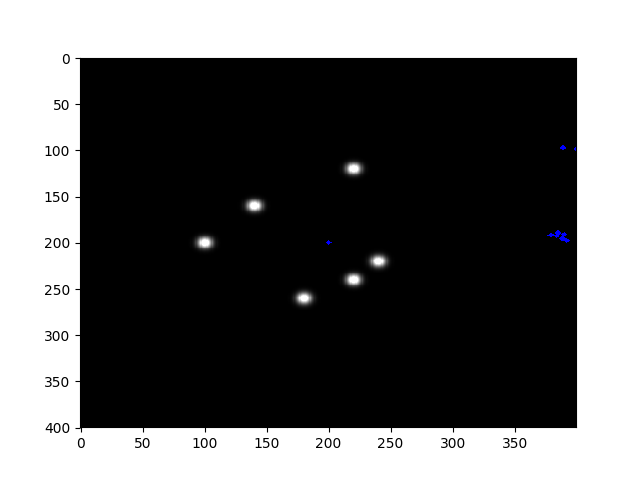
\includegraphics[height = 40mm,width = 60mm]{ML field.png}
        \end{subfigure}
    \end{figure}   


    \end{itemize}
\end{frame}


\subsection{Resampling}
\begin{frame}{Resampling}
    Various Resampling approaches were tried out -
    \begin{itemize}
        \item \textbf{Fitness proportion sampling:} Used the default resampler available in numpy \\
            \textit{numpy.random.choice(particles, num=N, p=weights)}
        \item \textbf{Roulette wheel selection :} Fitnesss values arranged as CDF around a wheel and a point is chosen at random
        \item \textbf{Stochastic Universal sampling :} Roulette wheel selection will be dominated by a few particles of highest fit. Some particles with high fitness values might be shadowed by the most fit members. This can result is global localisation failure. To avoid this SUS was tried. Though it reduces localisation failure, it can still result in localisation failure  
    \end{itemize}
\end{frame}

\begin{frame}{Resampling cont..}
    \begin{figure}
        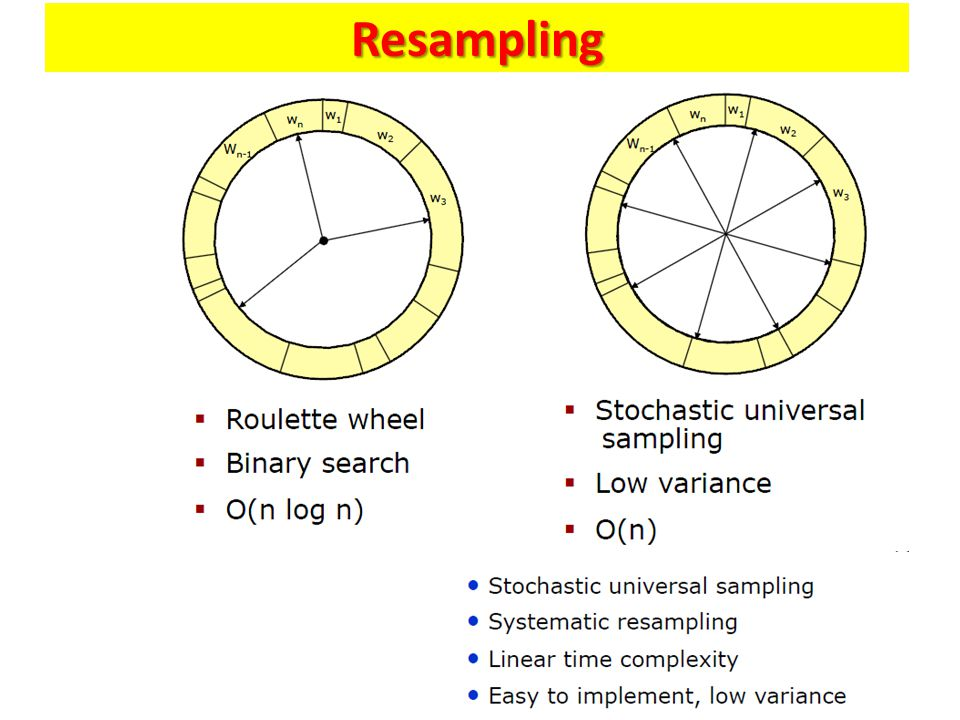
\includegraphics[height = 80mm]{./rl_multi.jpg}
        \caption{Particle structure in RBPF-slam}
    \end{figure}
\end{frame}


\section{Simulations}
\begin{frame}{Simulations}

    \begin{itemize}
        \item \href{https://github.com/aswinpajayan/seminar-related/blob/master/gifs/MCL-final.gif}{Particle localisation}
        \item \href{https://github.com/aswinpajayan/seminar-related/blob/master/gifs/sensorscans.gif}{Super imposed of ML field}
    \end{itemize}
\end{frame}


\begin{frame}{ROS node architecture}
\begin{figure}
        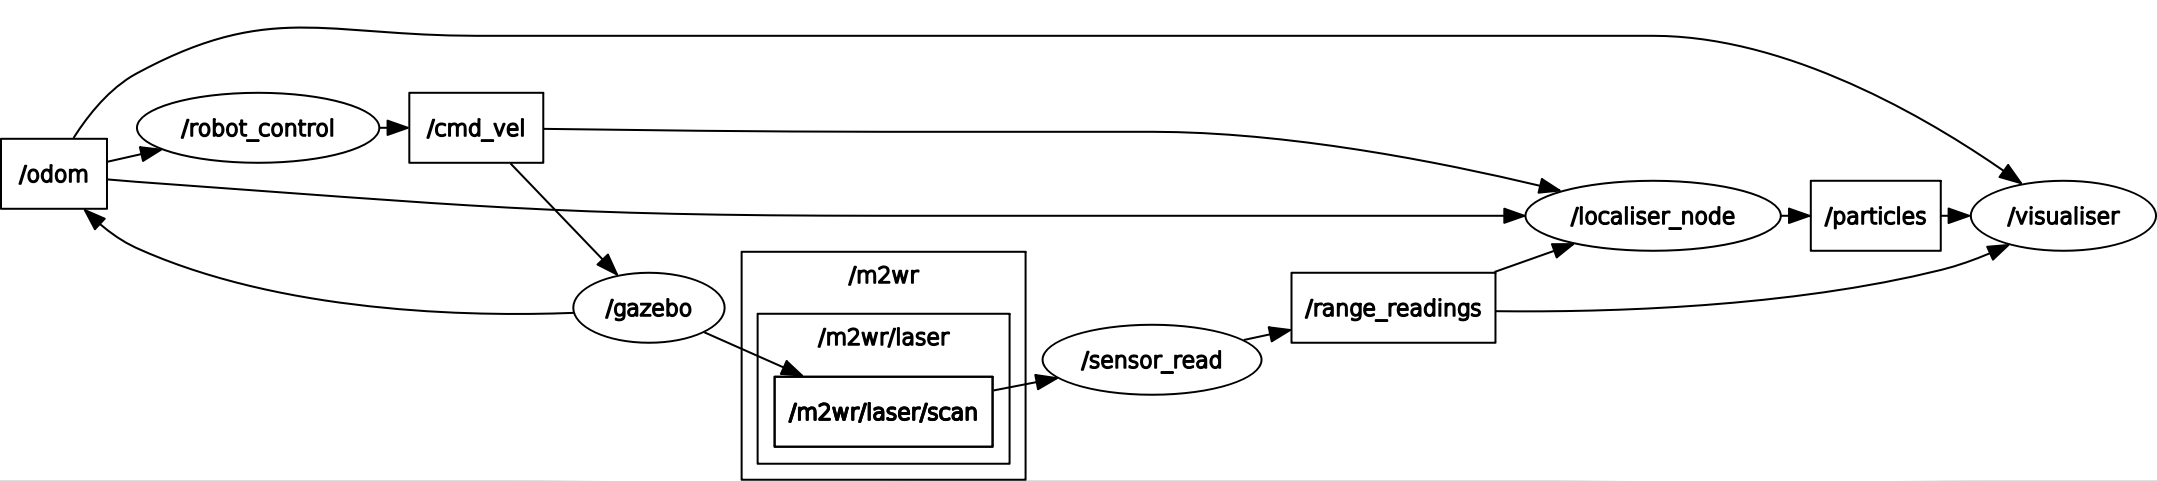
\includegraphics[width = 120mm]{./rosgraph.png}
        \caption{Ros graph generated using rqt\_graph}
    \end{figure}
\end{frame}

\begin{frame}{Physics simulations with gazebo}
\begin{figure}
    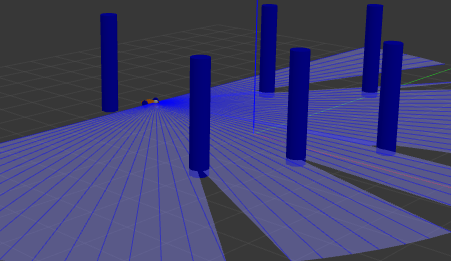
\includegraphics[width = 120mm]{./physics.png}
        \caption{Robot kinematics and sensor physics is taken care of by gazebo}
    \end{figure}
\end{frame}
% \begin{frame}{DLC384 Reading FSM Diagram}
%      \begin{figure}
%         \includegraphics[width = 100mm]{DLC384-reading-FSM.png}$^{8}$
%     \end{figure}   
% \end{frame}

\section{suggested improvements}
\begin{frame}{Suggested Improvements}
    \begin{itemize}
        \item Increasing the number of particles. Simualtions are quite heavy and the number of particles was limited by laptop hardware
        \item Better sampling strategy : Current resampling stratgy favours high fit particles to the extent that low fitness particles are often lost. Need a better resampling strategy to improve sampling.
        \item Augmented MCL to counter globalisation failures. Right now globalisation failure is countered by artificially inflating the sensor noise.
        \item Accurate kinematic model for the robot
    \end{itemize}
\end{frame}

\section{Code Organisation}
\begin{frame}{Code Organisation}
    The entire code can be found at github \href{https://github.com/aswinpajayan/localisation-mcl/tree/touchups}{link} in branch touchups
     \begin{itemize}
         \item ROS uses python 2.7. caktin\_make build system is used to build custom messages
         \item robot mesh and model descriptions are present in folder urdf
         \item launch file is used to initialise various ros nodes - present in launch folder (no\_ui\_spawn.launch)
         \item All scripts are found in scripts folder

            \begin{itemize}
                \item scripts/robot\_model.py contains kinematic and sensor models
                    \item scripts/read\_sensor.py contains node to handle hokuyo laser range finder and correspondence algorithm 
                    \item scripts/lv\_resample.py contains various resampling algorithms used
                    \item scripts/my\_MCL.py handles robot localisation
            \end{itemize}
     \end{itemize}
\end{frame}

\section{Appendix}
\subsection{PF algorithm}


\begin{frame}{MCL localisation algorithm}
    \begin{figure}
        \centering
        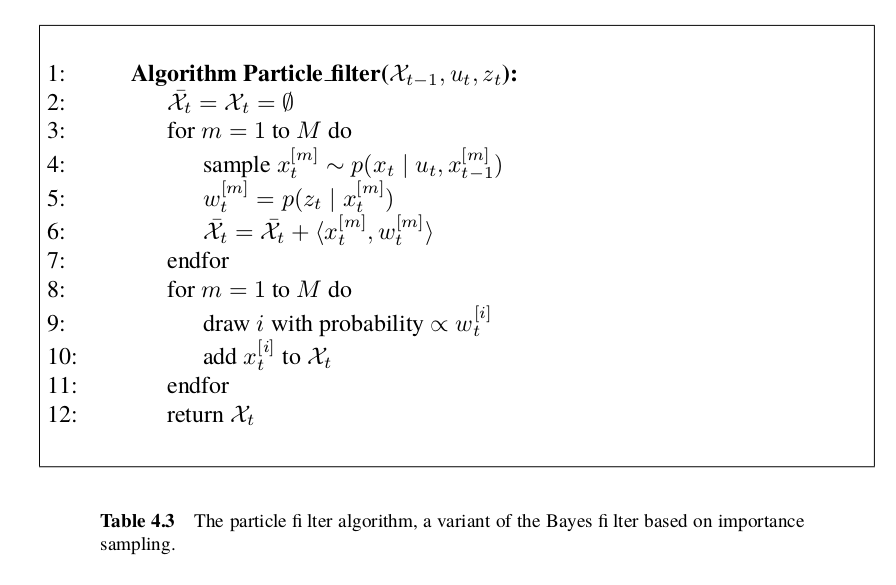
\includegraphics[width=\textwidth]{./PF.png}$^{1}$
    \end{figure}
\end{frame}

\subsection{Augmented MCL algorithm}
\begin{frame}{Augmented MCL algorithm}
    \begin{figure}
        \centering
        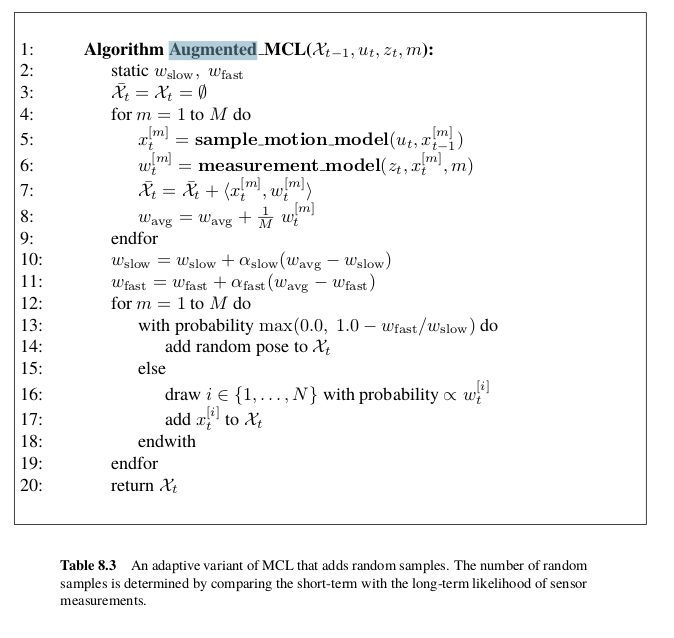
\includegraphics[height = 80mm]{./Augmented.png}$^{1}$
    \end{figure}
\end{frame}


\section{Future Work}
\begin{frame}{Future Work}
\begin{itemize}
    \item Perfect Localisation using Augmented MCL and low variance resampling
    \item Move on to implementing RBPF SLAM in ROS 
    \item Running ROS in client server mode offloading heavy computations to lab machine 
\end{itemize}
\end{frame}

\section{References}
\begin{frame}{References}
\begin{thebibliography}{}
\setbeamertemplate{bibliography item}[text]
\bibitem{1} Probabilistic Robotics by Sebastian Thrun
\bibitem{2} \href{https://www.youtube.com/playlist?list=PLgnQpQtFTOGQrZ4O5QzbIHgl3b1JHimN\_}{SLAM Lectures by Prof Cyrill Stachniss}
\bibitem{3} \href{https://www.theconstructsim.com/ros-projects-exploring-ros-using-2-wheeled-robot-part-1/}{URDF tutorials by construct sim}
\bibitem{4} \href{http://wiki.ros.org/ROS/Tutorials}{ROS wiki}
\bibitem{5} Simultaneous Localisation and Mapping (SLAM): Part I The Essential Algorithms By Hugh Durrant-Whyte
\end{thebibliography}
\end{frame}


\begin{frame}
\Huge{\centerline{Thank You for your Attention}}
\end{frame}

\end{document}
